\documentclass[12pt]{article}

\pagestyle{empty}
\setcounter{secnumdepth}{2}

\topmargin=0cm
\oddsidemargin=0cm
\textheight=22.0cm
\textwidth=16cm
\parindent=0cm
\parskip=0.15cm
\topskip=0truecm
\raggedbottom
\abovedisplayskip=3mm
\belowdisplayskip=3mm
\abovedisplayshortskip=0mm
\belowdisplayshortskip=2mm
\normalbaselineskip=12pt
\normalbaselines
\usepackage[table]{xcolor}
\usepackage{caption}
\usepackage{graphicx}
\usepackage{array}

\begin{document}

\graphicspath{{C:/Users/Marc/Desktop/ReqDocFolder/}}

\vspace*{0.5in}
\centerline{\bf\Large Requirements Document}

\vspace*{0.5in}
\centerline{\bf\Large Team PI-B}

\vspace*{0.5in}
\centerline{\bf\Large 9 February 2020}

\vspace*{1.0in}
\centerline{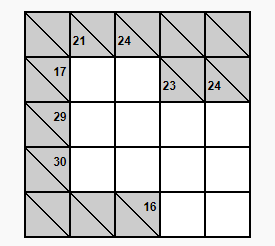
\includegraphics[scale=.75]{KakuroTemp.png}}
\centerline{\bf\Large Kakuro}

\vspace*{0.5in}
\begin{table}[htbp]
\begin{center}
\caption*{Team members}
\begin{tabular}{|c | c|}
\hline
\cellcolor{gray}Name & \cellcolor{gray}ID Number \\
\hline
Sajib Ahmed & A \\
\hline
Yaroslav Bilodid & B \\
\hline
Jesse Desmarais & C \\
\hline
Antoine Farley & D \\
\hline
Marc Hegedus & E \\
\hline
Katerina Tambakis & F \\
\hline
Dmytro Chychkov & G \\
\hline
Shuo Zhang & H \\
\hline
\end{tabular}
\end{center}
\end{table}

\clearpage

\section{System}

\subsection{Purpose}

\subsection{Context}

\subsection{Business Goals}

\section{Domain Concepts}

\section{Actors}

\section{Use Cases}

\subsection{Overview}

\begin{figure}[htbp]
%insert diagram here
\caption{Use Case Diagram}
\label{fig:use-case-diagram}
\end{figure}

\subsubsection{Use Case 1} \label{uc:1}

\noindent
{\bf Name}\\
Give a name.

\noindent
{\bf Summary}\\
A short summary/description/story.

\noindent
{\bf Actors}\\

\noindent
{\bf Precondition}\\

\noindent
{\bf Main Scenario}\\
\vspace*{-0.2in}
\begin{enumerate}
\item Describe step 1.
\item Describe step 2.
\item Describe step 3.
\end{enumerate}

\noindent
{\bf Exceptions}\\

\noindent
{\bf Postcondition}\\

\noindent
{\bf Priority}\\

\noindent
{\bf Traces to Test Cases}\\
Add when test cases done.

\subsubsection{Use Case 2} \label{uc:2}

\section{Non-Functional Constraints}

\section{Data Dictionary}

\section{References}

\appendix

\section{Description of File Format: Tasks}

Describe input file format.

\section{Description of File Format: Persons}

Describe output file format.

\end{document}
